\documentclass[10pt,a4paper]{article}
\usepackage{fullpage}
\usepackage[utf8]{inputenc}
\usepackage[english]{babel}
\usepackage[hidelinks]{hyperref}
\usepackage{amsmath}
\usepackage{amsfonts}
\usepackage{float}
\usepackage{subcaption}
\usepackage{tikz}
\usetikzlibrary{colorbrewer}
\usepackage{pgfplots}
\usepackage{pgfplotstable}
\pgfplotsset{compat=newest}
\usepgfplotslibrary{groupplots}
\usepgfplotslibrary{units}
% \usepgfplotslibrary{external}
% \tikzexternalize

\usepackage{mathrm}
\usepackage{mat-vec}

\definecolor{brewergreylight}{RGB}{224,224,224}
\definecolor{brewergrey}{RGB}{99,99,99}
\definecolor{brewerred}{RGB}{227,74,51}
\definecolor{brewerblue}{RGB}{33,113,181}
\definecolor{brewergreen}{RGB}{49,163,84}
\definecolor{brewergreendark}{RGB}{152,78,163}
\definecolor{breweryellow}{RGB}{27,120,55}

\listfiles

\begin{document}
\title{IGA of a Photocathode}
\date{}
\author{}
\maketitle

\tableofcontents

% \section{60 kV Geometry}
% \subsection{Geometry}
The $60$ kV geometry was derived from the technical drawings in \cite{espig}. Some simplifications were made especially regarding the inner part of the electrode, such that the geometry may be modeled as being rotationally symmetric. The dimensions of the electrode, puck, puck elevator, vacuum chamber and insulator were derived from Figure A.1, A.2, A.3, A.4 and A.6 in \cite{espig} respectively. The geometry of the vacuum chamber was also simplified to reduce the computational domain and the reduced insulator geometry is in part based on the drawing in Figure 5.7 of the thesis.
The boundary conditions were retrieved from Table 5.1 in \cite{espig} and the relative permittivity of the insulator was taken from an existing CST model to be $9.4$.

The geometry is depicted in fig.~\ref{fig:geometry} and a technical drawing of the actual geometry is given in fig.~\ref{fig:cad_geometry} for comparison. The numbers in the simplified geometry refer to the individual patches in the context of IGA. The patch boundaries are indicated by the black lines. The red lines represent homogeneous Dirichlet boundary conditions, the blue lines inhomogeneous Dirichlet boundary conditions with a value of $-60\ \mathrm{kV}$ and the green lines indicate homogeneous Neumann boundaries.
According to the technical drawings patch $10$ as well as parts of patches $7$ and $8$ are modeled as insulator material.

\begin{center}
\begin{figure}[H]
  \begin{tikzpicture}

\begin{axis}[
  enlargelimits=true,
  colormap/YlOrRd,
  point meta min = 0,
  point meta max = 5,
  x unit=m,
  y unit=m,
  legend pos=outer north east]

  \addplot[surf, shader=interp] table[point meta=\thisrow{c}]{figures/60kV/geometry/geometry_1.dat};

  \addplot[surf, shader=interp] table[point meta=\thisrow{c}]{figures/60kV/geometry/geometry_2.dat};

  \addplot[surf, shader=interp] table[point meta=\thisrow{c}]{figures/60kV/geometry/geometry_3.dat};

  \addplot[surf, shader=interp] table[point meta=\thisrow{c}]{figures/60kV/geometry/geometry_4.dat};

  \addplot[surf, shader=interp] table[point meta=\thisrow{c}]{figures/60kV/geometry/geometry_5.dat};

  \addplot[surf, shader=interp] table[point meta=\thisrow{c}]{figures/60kV/geometry/geometry_6.dat};

  \addplot[surf, shader=interp] table[point meta=\thisrow{c}]{figures/60kV/geometry/geometry_7.dat};

  \addplot[surf, shader=interp] table[point meta=\thisrow{c}]{figures/60kV/geometry/geometry_8.dat};

  \addplot[surf, shader=interp] table[point meta=\thisrow{c}]{figures/60kV/geometry/geometry_9.dat};

  \addplot[surf, shader=interp] table[point meta=\thisrow{c}]{figures/60kV/geometry/geometry_10.dat};

  \addplot[surf, shader=interp] table[point meta=\thisrow{c}]{figures/60kV/geometry/geometry_11.dat};

  \addplot[surf, shader=interp] table[point meta=\thisrow{c}]{figures/60kV/geometry/geometry_12.dat};

  \addplot[surf, shader=interp] table[point meta=\thisrow{c}]{figures/60kV/geometry/geometry_13.dat};

  /tikz/font=\normalfont\tiny
  % add patch indices
  \addplot[only marks, point meta=explicit symbolic, color=black, nodes near coords] coordinates{
  (0.14,-0.001) [(1)]
  (0.14,0.013) [(2)]
  (0.14,0.05) [(3)]
  (0.12,0.1) [(4)]
  (0.04,0.1) [(5)]
  (-0.025,0.06) [(6)]
  (-0.025,0.03) [(7)]
  (-0.021,0.02) [(8)]
  (-0.022,0.011) [(9)]
  (-0.025,0) [(10)]
  (0.016,0.012) [(11)]
  (0.027,0.017) [(12)]
  (0.055,0.021) [(13)]
  };

  % add patch boundaries
  \addplot[color=brewergreen, line width=1pt] table{figures/60kV/boundary/boundaries11.dat};
  \addplot[color=brewergrey] table{figures/60kV/boundary/boundaries12.dat};
  \addplot[color=brewerblue, line width=1pt] table{figures/60kV/boundary/boundaries13.dat};
  \addplot[color=brewerred, line width=1pt] table{figures/60kV/boundary/boundaries14.dat};

  \addplot[color=brewergrey] table{figures/60kV/boundary/boundaries21.dat};
  \addplot[color=brewergrey] table{figures/60kV/boundary/boundaries22.dat};
  \addplot[color=brewerblue, line width=1pt] table{figures/60kV/boundary/boundaries23.dat};
  \addplot[color=brewerred, line width=1pt] table{figures/60kV/boundary/boundaries24.dat};

  \addplot[color=brewergrey] table{figures/60kV/boundary/boundaries31.dat};
  \addplot[color=brewergrey] table{figures/60kV/boundary/boundaries32.dat};
  \addplot[color=brewerblue, line width=1pt] table{figures/60kV/boundary/boundaries33.dat};
  \addplot[color=brewerred, line width=1pt] table{figures/60kV/boundary/boundaries34.dat};

  \addplot[color=brewerblue, line width=1pt] table{figures/60kV/boundary/boundaries41.dat};
  \addplot[color=brewerred, line width=1pt] table{figures/60kV/boundary/boundaries42.dat};
  \addplot[color=brewergrey] table{figures/60kV/boundary/boundaries43.dat};
  \addplot[color=brewergrey] table{figures/60kV/boundary/boundaries44.dat};

  \addplot[color=brewerblue, line width=1pt] table{figures/60kV/boundary/boundaries51.dat};
  \addplot[color=brewerred, line width=1pt] table{figures/60kV/boundary/boundaries52.dat};
  \addplot[color=brewergrey] table{figures/60kV/boundary/boundaries53.dat};
  \addplot[color=brewergrey] table{figures/60kV/boundary/boundaries54.dat};

  \addplot[color=brewergrey] table{figures/60kV/boundary/boundaries61.dat};
  \addplot[color=brewergrey] table{figures/60kV/boundary/boundaries62.dat};
  \addplot[color=brewerred, line width=1pt] table{figures/60kV/boundary/boundaries63.dat};
  \addplot[color=brewerblue, line width=1pt] table{figures/60kV/boundary/boundaries64.dat};

  \addplot[color=brewergrey] table{figures/60kV/boundary/boundaries71.dat};
  \addplot[color=brewergrey] table{figures/60kV/boundary/boundaries72.dat};
  \addplot[color=brewerred, line width=1pt] table{figures/60kV/boundary/boundaries73.dat};
  \addplot[color=brewerblue, line width=1pt] table{figures/60kV/boundary/boundaries74.dat};

  \addplot[color=brewergrey] table{figures/60kV/boundary/boundaries81.dat};
  \addplot[color=brewergrey] table{figures/60kV/boundary/boundaries82.dat};
  \addplot[color=brewerred, line width=1pt] table{figures/60kV/boundary/boundaries83.dat};
  \addplot[color=brewerblue, line width=1pt] table{figures/60kV/boundary/boundaries84.dat};

  \addplot[color=brewergrey] table{figures/60kV/boundary/boundaries91.dat};
  \addplot[color=brewergrey] table{figures/60kV/boundary/boundaries92.dat};
  \addplot[color=brewerred, line width=1pt] table{figures/60kV/boundary/boundaries93.dat};
  \addplot[color=brewergrey] table{figures/60kV/boundary/boundaries94.dat};

  \addplot[color=brewergreen, line width=1pt] table{figures/60kV/boundary/boundaries101.dat};
  \addplot[color=brewergrey] table{figures/60kV/boundary/boundaries102.dat};
  \addplot[color=brewerred, line width=1pt] table{figures/60kV/boundary/boundaries103.dat};
  \addplot[color=brewerblue, line width=1pt] table{figures/60kV/boundary/boundaries104.dat};

  \addplot[color=brewerblue, line width=1pt] table{figures/60kV/boundary/boundaries111.dat};
  \addplot[color=brewerblue, line width=1pt] table{figures/60kV/boundary/boundaries112.dat};
  \addplot[color=brewergrey] table{figures/60kV/boundary/boundaries113.dat};
  \addplot[color=brewergrey] table{figures/60kV/boundary/boundaries114.dat};

  \addplot[color=brewergrey] table{figures/60kV/boundary/boundaries121.dat};
  \addplot[color=brewergrey] table{figures/60kV/boundary/boundaries122.dat};
  \addplot[color=brewerblue, line width=1pt] table{figures/60kV/boundary/boundaries123.dat};
  \addplot[color=brewerblue, line width=1pt] table{figures/60kV/boundary/boundaries124.dat};

  \addplot[color=brewerblue, line width=1pt] table{figures/60kV/boundary/boundaries131.dat};
  \addplot[color=brewerblue, line width=1pt] table{figures/60kV/boundary/boundaries132.dat};
  \addplot[color=brewergrey] table{figures/60kV/boundary/boundaries133.dat};
  \addplot[color=brewerblue, line width=1pt] table{figures/60kV/boundary/boundaries134.dat};

\end{axis}
\end{tikzpicture}

  \caption{60 kV Photocathode geometry and boundary conditions.}
  \label{fig:geometry}
\end{figure}
\end{center}

\begin{center}
\begin{figure}[H]
  \includegraphics[width=\textwidth]{figures/60kV/geometry}
  \caption{Part of the CAD drawing of the geometry.}
  \label{fig:cad_geometry}
\end{figure}
\end{center}

\subsection{Electrostatic Potential and Electric Field}
\label{sec:potential_field}
The solution for the electrostatic potential is shown in fig.~\ref{fig:potential}. Fig.~\ref{fig:electric_field} depicts the absolute value of the electric field.
Both of the solutions were computed with $p=4$ as the degree of the basis functions and $n_\mathrm{sub}=128$ as the number of elements that each knot vector is uniformly split into.
To give a comparison with the previous simulations fig.~\ref{fig:phd_electric_field} shows the results depicted in the thesis \cite{espig}. It is visible that the solutions are similar with the peak values appearing near the circular parts of the electrode. However the new results indicate that the absolute largest values occur at the back of the electrode and they also show higher field magnitudes in the insulator regions. This is a clear contrast to the previous simulation.
A second comparison can be made with the updated CST model from fig.~\ref{fig:electric_field_wende} from \cite{wende}. The absolute largest field values appear in the same region, however their magnitude is higher.
The bevavior of the field at the triple point is also very similar in that the surrounding magnitudes are very small.

\begin{center}
\begin{figure}[H]
  \includegraphics[width=\textwidth]{figures/60kV/potential}
  \caption{Electrostatic potential.}
  \label{fig:potential}
\end{figure}
\end{center}

\begin{center}
\begin{figure}[H]
  \includegraphics[width=\textwidth]{figures/60kV/gradient}
  \caption{Absolute value of the electric field.}
  \label{fig:electric_field}
\end{figure}
\end{center}

\begin{center}
\begin{figure}[H]
  \includegraphics[width=\textwidth]{figures/60kV/electric_field}
  \caption{Results from the PhD thesis.}
  \label{fig:phd_electric_field}
\end{figure}
\end{center}

\begin{center}
\begin{figure}[H]
  \includegraphics[width=\textwidth]{figures/60kV/electric_field_wende}
  \caption{Results from the Bachelor thesis.}
  \label{fig:electric_field_wende}
\end{figure}
\end{center}

\subsection{Convergence Study}
The convergence studies investigate the accuracy of the solution while increasing the number of elements per patch. (Akin to $h$-refinement in classical FEA) Since no analytic solution exists we used a reference with $n_\mathrm{sub}=256$ and $p=4$ as a comparison.
The errors are computed as
\begin{align}
  e_{L^2} = \frac{\| \varphi_\mathrm{it} - \varphi_\mathrm{ref} \|_{L^2}}{\| \varphi_\mathrm{ref} \|_{L^2}}\\
  e_{H^1} = \frac{\| \varphi_\mathrm{it} - \varphi_\mathrm{ref} \|_{H^1}}{\| \varphi_\mathrm{ref} \|_{H^1}}
\end{align}
where
\begin{align}
  \| \varphi \|_{H^1} = \sqrt{ \| \varphi \|_{L^2}^2 + \| \nabla\varphi \|_{L^2}^2 }.
\end{align}
Here $\varphi$ denotes the electrostatic potential. The integrals associated with the $L^2$-norm are evaluated using a quadrature rule defined on each element of a given patch.

The degrees of the basis functions are given in the legend, as well as theoretical limits for the convergence rates. They are given by $p+1$ in the case of the $L^2$-norm (electrostatic potential) and $p$ in the case of the $H^1$-norm (electric field). As seen in fig.~\ref{fig:convergence_potential} and fig.~\ref{fig:convergence_gradient} we observe convergence, however the convergence rate appears to be limited.

\begin{figure}[H]
  \begin{center}
    \begin{tikzpicture}

\begin{loglogaxis}[
  xlabel={$1/nsub$},
  ylabel={relative error},
  legend entries={$p=2$, $h^{2+1}$, $p=3$, $h^{3+1}$, $p=4$, $h^{4+1}$},
  legend pos=outer north east]

\addplot [color=brewerred] table[x=h, y=errl2]{figures/insulator/convergence/convergence_ref=5_degree=2.dat};

\addplot [color=brewergrey] table[x=h, y=h_l2]{figures/insulator/convergence/convergence_ref=5_degree=2.dat};

\addplot [color=brewerblue] table[x=h, y=errl2]{figures/insulator/convergence/convergence_ref=5_degree=3.dat};

\addplot [color=brewergrey] table[x=h, y=h_l2]{figures/insulator/convergence/convergence_ref=5_degree=3.dat};

\addplot [color=brewergreen] table[x=h, y=errl2]{figures/insulator/convergence/convergence_ref=5_degree=4.dat};

\addplot [color=brewergrey] table[x=h, y=h_l2]{figures/insulator/convergence/convergence_ref=5_degree=4.dat};

\end{loglogaxis}
\end{tikzpicture}

    \caption{Convergence of $L^2$-norm.}
    \label{fig:convergence_potential}
  \end{center}
\end{figure}

\begin{figure}[H]
  \begin{center}
    \begin{tikzpicture}

\begin{loglogaxis}[
  xlabel={$1/nsub$},
  ylabel={relative error},
  legend entries={$p=2$, $h^{2}$, $p=3$, $h^{3}$, $p=4$, $h^{4}$},
  legend pos=outer north east]

\addplot [color=brewerred] table[x=h, y=errh1]{figures/insulator/convergence/convergence_ref=5_degree=2.dat};

\addplot [color=brewergrey] table[x=h, y=h_h1]{figures/insulator/convergence/convergence_ref=5_degree=2.dat};

\addplot [color=brewerblue] table[x=h, y=errh1]{figures/insulator/convergence/convergence_ref=5_degree=3.dat};

\addplot [color=brewergrey] table[x=h, y=h_h1]{figures/insulator/convergence/convergence_ref=5_degree=3.dat};

\addplot [color=brewergreen] table[x=h, y=errh1]{figures/insulator/convergence/convergence_ref=5_degree=4.dat};

\addplot [color=brewergrey] table[x=h, y=h_h1]{figures/insulator/convergence/convergence_ref=5_degree=4.dat};

\end{loglogaxis}
\end{tikzpicture}

    \caption{Convergence of $H^1$-norm.}
    \label{fig:convergence_gradient}
  \end{center}
\end{figure}

Lastly the error in specific regions of the geometry was investigated by displaying the absolute error of the eletric field on every individual element of the mesh. In the case of fig.~\ref{fig:error_elem} we chose $n_\mathrm{sub}=256$ and $p=3$ for the iterative solution and computed the errors with respect to a reference using $n_\mathrm{sub}=256$ and $p=4$.
The figure shows the absolute error on each element in a logarithmic scale. We observe that the errors are largest near sharp corners or large changes in the sizes of the mesh's elements. This is to be expected and as indicated by the colorbar the largest absolute errors come out to be around $19\ \mathrm{V/m}$ with the associated field magnitudes being almost exclusively larger than $10\ \mathrm{MV/m}$.

\begin{center}
\begin{figure}[H]
  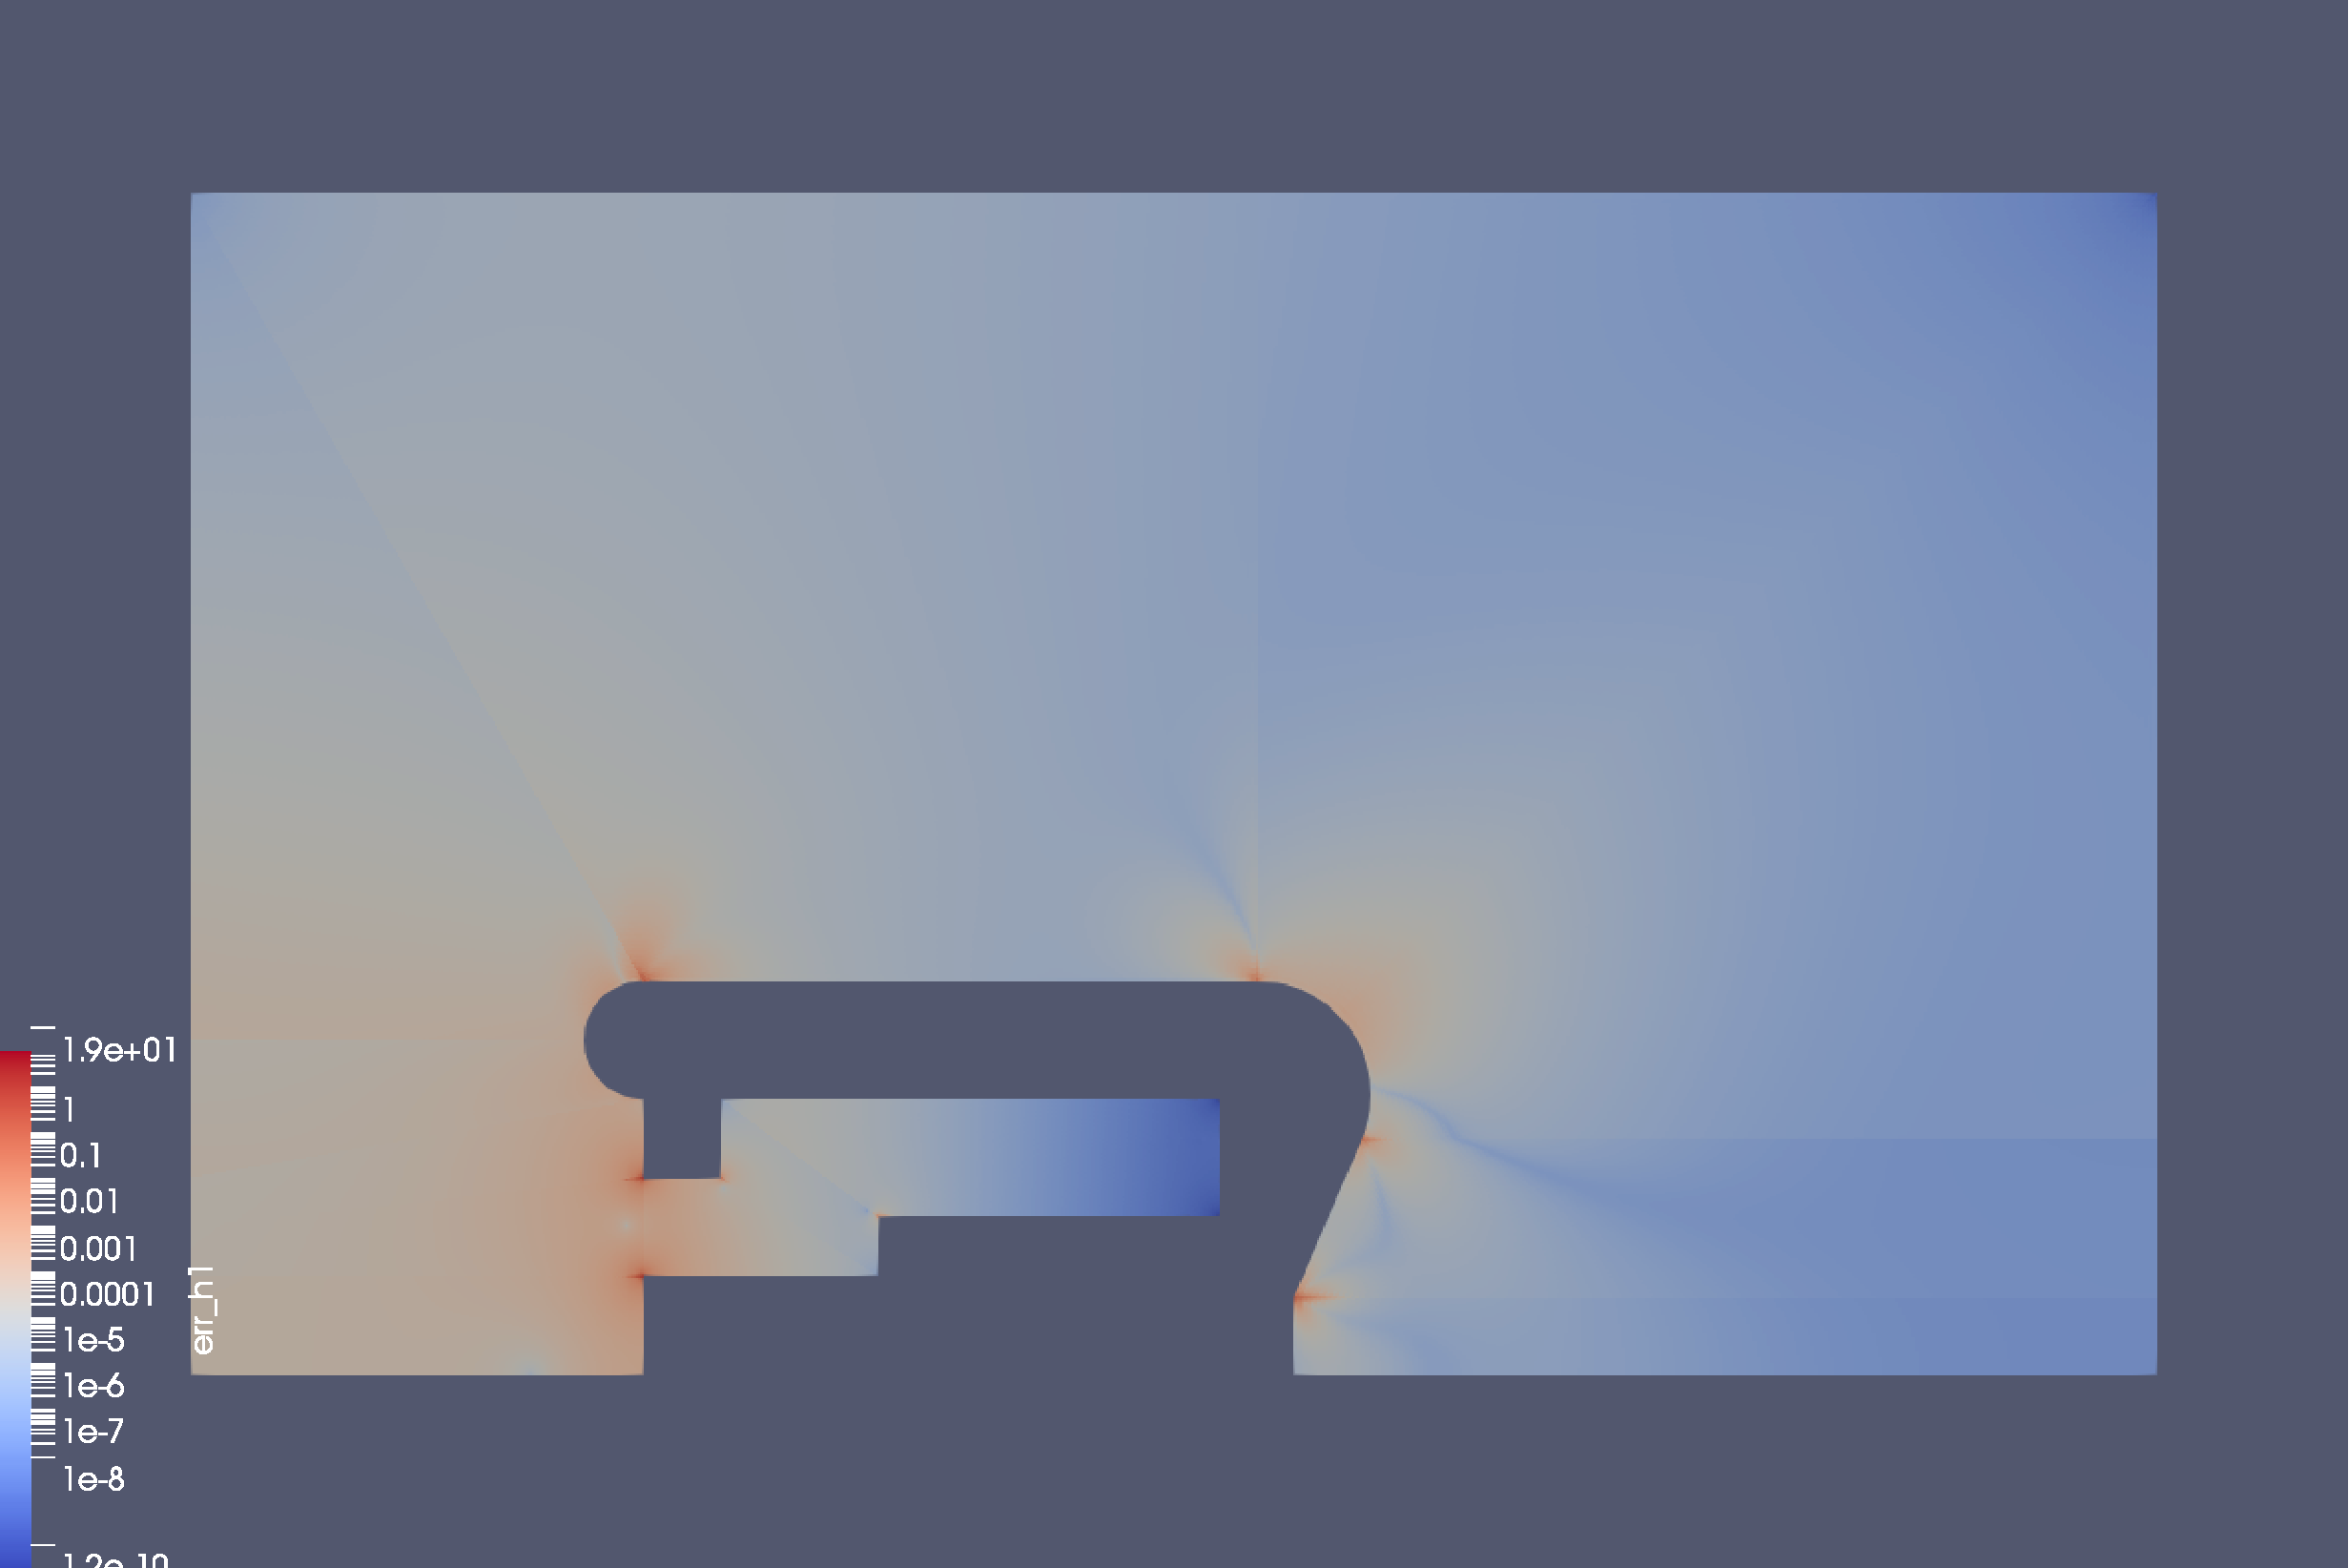
\includegraphics[width=\textwidth]{figures/60kV/error_elem}
  \caption{Absolute error of the electric field on every element.}
  \label{fig:error_elem}
\end{figure}
\end{center}


\section{200 kV Geometry}
\subsection{Geometry}
The $200$ kV geometry was derived from version one of the CST model. Some simplifications were made such that the geometry may be considered rotationally symmetric. The dimensions of the electrode, puck, puck elevator, vacuum chamber and insulator were derived from the model as depicted in fig.~\ref{fig:cst_geometry_yz}. The boundary conditions remained the same, except for the increase in voltage, when compared to the $60$ kV variant and the relative permittivity of the insulator was taken from the model to be $9.4$.

The geometry is depicted in fig.~\ref{fig:200kV_geometry}. The numbers refer to the individual patches in the context of IGA. The patch boundaries are indicated by grey lines. The red lines represent homogeneous Dirichlet boundary conditions, the blue lines inhomogeneous Dirichlet boundary conditions with a value of $-200$ kV and the black lines indicate homogeneous Neumann boundaries.
The patches containing insulator material are colored in red.

\begin{center}
\begin{figure}[H]
  \includegraphics[width=\textwidth]{figures/200kV/v1_cutx}
  \caption{$y$-$z$ view of the CST model for $x=0$.}
  \label{fig:cst_geometry_yz}
\end{figure}
\end{center}

\begin{center}
\begin{figure}[H]
  % \begin{tikzpicture}

\begin{axis}[
  enlargelimits=true,
  colormap/YlOrRd,
  point meta min = 0,
  point meta max = 5,
  x unit=m,
  y unit=m,
  legend pos=outer north east]

  \addplot[surf, shader=interp] table[point meta=\thisrow{c}]{figures/60kV/geometry/geometry_1.dat};

  \addplot[surf, shader=interp] table[point meta=\thisrow{c}]{figures/60kV/geometry/geometry_2.dat};

  \addplot[surf, shader=interp] table[point meta=\thisrow{c}]{figures/60kV/geometry/geometry_3.dat};

  \addplot[surf, shader=interp] table[point meta=\thisrow{c}]{figures/60kV/geometry/geometry_4.dat};

  \addplot[surf, shader=interp] table[point meta=\thisrow{c}]{figures/60kV/geometry/geometry_5.dat};

  \addplot[surf, shader=interp] table[point meta=\thisrow{c}]{figures/60kV/geometry/geometry_6.dat};

  \addplot[surf, shader=interp] table[point meta=\thisrow{c}]{figures/60kV/geometry/geometry_7.dat};

  \addplot[surf, shader=interp] table[point meta=\thisrow{c}]{figures/60kV/geometry/geometry_8.dat};

  \addplot[surf, shader=interp] table[point meta=\thisrow{c}]{figures/60kV/geometry/geometry_9.dat};

  \addplot[surf, shader=interp] table[point meta=\thisrow{c}]{figures/60kV/geometry/geometry_10.dat};

  \addplot[surf, shader=interp] table[point meta=\thisrow{c}]{figures/60kV/geometry/geometry_11.dat};

  \addplot[surf, shader=interp] table[point meta=\thisrow{c}]{figures/60kV/geometry/geometry_12.dat};

  \addplot[surf, shader=interp] table[point meta=\thisrow{c}]{figures/60kV/geometry/geometry_13.dat};

  /tikz/font=\normalfont\tiny
  % add patch indices
  \addplot[only marks, point meta=explicit symbolic, color=black, nodes near coords] coordinates{
  (0.14,-0.001) [(1)]
  (0.14,0.013) [(2)]
  (0.14,0.05) [(3)]
  (0.12,0.1) [(4)]
  (0.04,0.1) [(5)]
  (-0.025,0.06) [(6)]
  (-0.025,0.03) [(7)]
  (-0.021,0.02) [(8)]
  (-0.022,0.011) [(9)]
  (-0.025,0) [(10)]
  (0.016,0.012) [(11)]
  (0.027,0.017) [(12)]
  (0.055,0.021) [(13)]
  };

  % add patch boundaries
  \addplot[color=brewergreen, line width=1pt] table{figures/60kV/boundary/boundaries11.dat};
  \addplot[color=brewergrey] table{figures/60kV/boundary/boundaries12.dat};
  \addplot[color=brewerblue, line width=1pt] table{figures/60kV/boundary/boundaries13.dat};
  \addplot[color=brewerred, line width=1pt] table{figures/60kV/boundary/boundaries14.dat};

  \addplot[color=brewergrey] table{figures/60kV/boundary/boundaries21.dat};
  \addplot[color=brewergrey] table{figures/60kV/boundary/boundaries22.dat};
  \addplot[color=brewerblue, line width=1pt] table{figures/60kV/boundary/boundaries23.dat};
  \addplot[color=brewerred, line width=1pt] table{figures/60kV/boundary/boundaries24.dat};

  \addplot[color=brewergrey] table{figures/60kV/boundary/boundaries31.dat};
  \addplot[color=brewergrey] table{figures/60kV/boundary/boundaries32.dat};
  \addplot[color=brewerblue, line width=1pt] table{figures/60kV/boundary/boundaries33.dat};
  \addplot[color=brewerred, line width=1pt] table{figures/60kV/boundary/boundaries34.dat};

  \addplot[color=brewerblue, line width=1pt] table{figures/60kV/boundary/boundaries41.dat};
  \addplot[color=brewerred, line width=1pt] table{figures/60kV/boundary/boundaries42.dat};
  \addplot[color=brewergrey] table{figures/60kV/boundary/boundaries43.dat};
  \addplot[color=brewergrey] table{figures/60kV/boundary/boundaries44.dat};

  \addplot[color=brewerblue, line width=1pt] table{figures/60kV/boundary/boundaries51.dat};
  \addplot[color=brewerred, line width=1pt] table{figures/60kV/boundary/boundaries52.dat};
  \addplot[color=brewergrey] table{figures/60kV/boundary/boundaries53.dat};
  \addplot[color=brewergrey] table{figures/60kV/boundary/boundaries54.dat};

  \addplot[color=brewergrey] table{figures/60kV/boundary/boundaries61.dat};
  \addplot[color=brewergrey] table{figures/60kV/boundary/boundaries62.dat};
  \addplot[color=brewerred, line width=1pt] table{figures/60kV/boundary/boundaries63.dat};
  \addplot[color=brewerblue, line width=1pt] table{figures/60kV/boundary/boundaries64.dat};

  \addplot[color=brewergrey] table{figures/60kV/boundary/boundaries71.dat};
  \addplot[color=brewergrey] table{figures/60kV/boundary/boundaries72.dat};
  \addplot[color=brewerred, line width=1pt] table{figures/60kV/boundary/boundaries73.dat};
  \addplot[color=brewerblue, line width=1pt] table{figures/60kV/boundary/boundaries74.dat};

  \addplot[color=brewergrey] table{figures/60kV/boundary/boundaries81.dat};
  \addplot[color=brewergrey] table{figures/60kV/boundary/boundaries82.dat};
  \addplot[color=brewerred, line width=1pt] table{figures/60kV/boundary/boundaries83.dat};
  \addplot[color=brewerblue, line width=1pt] table{figures/60kV/boundary/boundaries84.dat};

  \addplot[color=brewergrey] table{figures/60kV/boundary/boundaries91.dat};
  \addplot[color=brewergrey] table{figures/60kV/boundary/boundaries92.dat};
  \addplot[color=brewerred, line width=1pt] table{figures/60kV/boundary/boundaries93.dat};
  \addplot[color=brewergrey] table{figures/60kV/boundary/boundaries94.dat};

  \addplot[color=brewergreen, line width=1pt] table{figures/60kV/boundary/boundaries101.dat};
  \addplot[color=brewergrey] table{figures/60kV/boundary/boundaries102.dat};
  \addplot[color=brewerred, line width=1pt] table{figures/60kV/boundary/boundaries103.dat};
  \addplot[color=brewerblue, line width=1pt] table{figures/60kV/boundary/boundaries104.dat};

  \addplot[color=brewerblue, line width=1pt] table{figures/60kV/boundary/boundaries111.dat};
  \addplot[color=brewerblue, line width=1pt] table{figures/60kV/boundary/boundaries112.dat};
  \addplot[color=brewergrey] table{figures/60kV/boundary/boundaries113.dat};
  \addplot[color=brewergrey] table{figures/60kV/boundary/boundaries114.dat};

  \addplot[color=brewergrey] table{figures/60kV/boundary/boundaries121.dat};
  \addplot[color=brewergrey] table{figures/60kV/boundary/boundaries122.dat};
  \addplot[color=brewerblue, line width=1pt] table{figures/60kV/boundary/boundaries123.dat};
  \addplot[color=brewerblue, line width=1pt] table{figures/60kV/boundary/boundaries124.dat};

  \addplot[color=brewerblue, line width=1pt] table{figures/60kV/boundary/boundaries131.dat};
  \addplot[color=brewerblue, line width=1pt] table{figures/60kV/boundary/boundaries132.dat};
  \addplot[color=brewergrey] table{figures/60kV/boundary/boundaries133.dat};
  \addplot[color=brewerblue, line width=1pt] table{figures/60kV/boundary/boundaries134.dat};

\end{axis}
\end{tikzpicture}

  \caption{200 kV Photocathode geometry and boundary conditions.}
  \label{fig:200kV_geometry}
\end{figure}
\end{center}

\begin{center}
\begin{figure}[H]
  \begin{tikzpicture}
\begin{axis}[
   scale only axis = true,
   width = 0.9\textwidth,
  axis equal,
  try min ticks=4,
  max space between ticks=1000pt,
  enlargelimits=true,
  colormap/Greys,
  point meta min = 0,
  point meta max = 3,
  x unit=m,
  y unit=m]

  \addplot[surf, shader=interp] table[point meta=\thisrow{c}]{figures/200kV/geometry/v3/geometry1.dat};

  \addplot[surf, shader=interp] table[point meta=\thisrow{c}]{figures/200kV/geometry/v3/geometry2.dat};

  \addplot[surf, shader=interp] table[point meta=\thisrow{c}]{figures/200kV/geometry/v3/geometry3.dat};

  \addplot[surf, shader=interp] table[point meta=\thisrow{c}]{figures/200kV/geometry/v3/geometry4.dat};

  \addplot[surf, shader=interp] table[point meta=\thisrow{c}]{figures/200kV/geometry/v3/geometry5.dat};

  \addplot[surf, shader=interp] table[point meta=\thisrow{c}]{figures/200kV/geometry/v3/geometry6.dat};

  \addplot[surf, shader=interp] table[point meta=\thisrow{c}]{figures/200kV/geometry/v3/geometry7.dat};

  \addplot[surf, shader=interp] table[point meta=\thisrow{c}]{figures/200kV/geometry/v3/geometry8.dat};

  \addplot[surf, shader=interp] table[point meta=\thisrow{c}]{figures/200kV/geometry/v3/geometry9.dat};

  \addplot[surf, shader=interp] table[point meta=\thisrow{c}]{figures/200kV/geometry/v3/geometry10.dat};

  \addplot[surf, shader=interp] table[point meta=\thisrow{c}]{figures/200kV/geometry/v3/geometry11.dat};

  \addplot[surf, shader=interp] table[point meta=\thisrow{c}]{figures/200kV/geometry/v3/geometry12.dat};

  \addplot[surf, shader=interp] table[point meta=\thisrow{c}]{figures/200kV/geometry/v3/geometry13.dat};

  \addplot[surf, shader=interp, colormap/Reds, point meta min = 0, point meta max = 1] table[point meta=\thisrow{c}]{figures/200kV/geometry/v3/geometry13.dat};

  \addplot[surf, shader=interp] table[point meta=\thisrow{c}]{figures/200kV/geometry/v3/geometry14.dat};

  \addplot[surf, shader=interp, colormap/Reds, point meta min = 0, point meta max = 1] table[point meta=\thisrow{c}]{figures/200kV/geometry/v3/geometry15.dat};

  \addplot[surf, shader=interp, colormap/Reds, point meta min = 0, point meta max = 1] table[point meta=\thisrow{c}]{figures/200kV/geometry/v3/geometry16.dat};

  \addplot[surf, shader=interp, colormap/Blues, point meta min = 0, point meta max = 1] table[point meta=\thisrow{c}]{figures/200kV/geometry/v3/geometry17.dat};

  \addplot[surf, shader=interp, colormap/Reds, point meta min = 0, point meta max = 1] table[point meta=\thisrow{c}]{figures/200kV/geometry/v3/geometry18.dat};

  \addplot[surf, shader=interp, colormap/Reds, point meta min = 0, point meta max = 1] table[point meta=\thisrow{c}]{figures/200kV/geometry/v3/geometry19.dat};

  \addplot[surf, shader=interp, colormap/Reds, point meta min = 0, point meta max = 1] table[point meta=\thisrow{c}]{figures/200kV/geometry/v3/geometry20.dat};

  \addplot[surf, shader=interp, colormap/Reds, point meta min = 0, point meta max = 1] table[point meta=\thisrow{c}]{figures/200kV/geometry/v3/geometry21.dat};

  \addplot[surf, shader=interp] table[point meta=\thisrow{c}]{figures/200kV/geometry/v3/geometry22.dat};

  \addplot[surf, shader=interp] table[point meta=\thisrow{c}]{figures/200kV/geometry/v3/geometry23.dat};

  \addplot[surf, shader=interp] table[point meta=\thisrow{c}]{figures/200kV/geometry/v3/geometry24.dat};

  \addplot[surf, shader=interp] table[point meta=\thisrow{c}]{figures/200kV/geometry/v3/geometry25.dat};

  \addplot[surf, shader=interp] table[point meta=\thisrow{c}]{figures/200kV/geometry/v3/geometry26.dat};

  \addplot[surf, shader=interp] table[point meta=\thisrow{c}]{figures/200kV/geometry/v3/geometry27.dat};

  \addplot[surf, shader=interp, colormap/Greens, point meta min = 0, point meta max = 1] table[point meta=\thisrow{c}]{figures/200kV/geometry/v3/geometry28.dat};

  \addplot[surf, shader=interp, colormap/Greens, point meta min = 0, point meta max = 1] table[point meta=\thisrow{c}]{figures/200kV/geometry/v3/geometry29.dat};

  \addplot[surf, shader=interp] table[point meta=\thisrow{c}]{figures/200kV/geometry/v3/geometry30.dat};

  \addplot[surf, shader=interp] table[point meta=\thisrow{c}]{figures/200kV/geometry/v3/geometry31.dat};

  \addplot[surf, shader=interp] table[point meta=\thisrow{c}]{figures/200kV/geometry/v3/geometry32.dat};

  \addplot[surf, shader=interp, colormap/Greens, point meta min = 0, point meta max = 1] table[point meta=\thisrow{c}]{figures/200kV/geometry/v3/geometry33.dat};

  \addplot[surf, shader=interp, colormap/Greens, point meta min = 0, point meta max = 1] table[point meta=\thisrow{c}]{figures/200kV/geometry/v3/geometry34.dat};

  \addplot[surf, shader=interp] table[point meta=\thisrow{c}]{figures/200kV/geometry/v3/geometry35.dat};

  \addplot[surf, shader=interp] table[point meta=\thisrow{c}]{figures/200kV/geometry/v3/geometry36.dat};

  \addplot[surf, shader=interp] table[point meta=\thisrow{c}]{figures/200kV/geometry/v3/geometry37.dat};

  \addplot[surf, shader=interp] table[point meta=\thisrow{c}]{figures/200kV/geometry/v3/geometry38.dat};

  \addplot[surf, shader=interp] table[point meta=\thisrow{c}]{figures/200kV/geometry/v3/geometry39.dat};

  % add patch indices
  \addplot[only marks, point meta=explicit symbolic, color=black, nodes near coords] coordinates{
  (0.235,-0.007) [1]
  (0.33,-0.007) [2]
  (0.235, -0.002) [3]
  (0.33, -0.002) [4]
  (0.235, 0.005) [5]
  (0.33, 0.005) [6]
  (0.235, 0.015) [7]
  (0.33, 0.017) [8]
  (0.235, 0.027) [9]
  (0.33, 0.035) [10]
  (0.235, 0.042) [11]
  (0.33, 0.057) [12]
  (0.26, 0.083) [13]
  (0.33, 0.083) [14]
  (0.212, 0.083) [15]
  (0.185, 0.083) [16]
  (0.158, 0.083) [17]
  (0.132, 0.083) [18]
  (0.103, 0.077) [19]
  (0.087, 0.058) [20]
  (0.094, 0.045) [21]
  (0.02, 0.09) [22]
  (0.065, 0.09) [23]
  (0.02, 0.062) [24]
  (0.055, 0.062) [25]
  (0.02, 0.048) [26]
  (0.055, 0.048) [27]
  (0.02, 0.034) [28]
  (0.062, 0.034) [29]
  (0.017, 0.022) [30]
  (0.062, 0.022) [31]
  (0.006, 0.012) [32]
  (0.062, 0.009) [33]
  (0.006, 0.006) [34]
  (0.035, -0.002) [35]
  (0.11, 0.022) [36]
  (0.178, 0.016) [37]
  (0.14, 0.022) [38]
  (0.158, 0.032) [39]
  };

  % add patch boundaries
  \addplot[color=brewerblue] table{figures/200kV/boundary/v3/boundaries11.dat};
  \addplot[color=brewergrey] table{figures/200kV/boundary/v3/boundaries12.dat};
  \addplot[color=black] table{figures/200kV/boundary/v3/boundaries13.dat};
  \addplot[color=brewergrey] table{figures/200kV/boundary/v3/boundaries14.dat};

  \addplot[color=brewergrey] table{figures/200kV/boundary/v3/boundaries21.dat};
  \addplot[color=brewerred] table{figures/200kV/boundary/v3/boundaries22.dat};
  \addplot[color=black] table{figures/200kV/boundary/v3/boundaries23.dat};
  \addplot[color=brewergrey] table{figures/200kV/boundary/v3/boundaries24.dat};

  \addplot[color=brewerblue] table{figures/200kV/boundary/v3/boundaries31.dat};
  \addplot[color=brewergrey] table{figures/200kV/boundary/v3/boundaries32.dat};
  \addplot[color=brewergrey] table{figures/200kV/boundary/v3/boundaries33.dat};
  \addplot[color=brewergrey] table{figures/200kV/boundary/v3/boundaries34.dat};

  \addplot[color=brewergrey] table{figures/200kV/boundary/v3/boundaries41.dat};
  \addplot[color=brewerred] table{figures/200kV/boundary/v3/boundaries42.dat};
  \addplot[color=brewergrey] table{figures/200kV/boundary/v3/boundaries43.dat};
  \addplot[color=brewergrey] table{figures/200kV/boundary/v3/boundaries44.dat};

  \addplot[color=brewerblue] table{figures/200kV/boundary/v3/boundaries51.dat};
  \addplot[color=brewergrey] table{figures/200kV/boundary/v3/boundaries52.dat};
  \addplot[color=brewergrey] table{figures/200kV/boundary/v3/boundaries53.dat};
  \addplot[color=brewergrey] table{figures/200kV/boundary/v3/boundaries54.dat};

  \addplot[color=brewergrey] table{figures/200kV/boundary/v3/boundaries61.dat};
  \addplot[color=brewerred] table{figures/200kV/boundary/v3/boundaries62.dat};
  \addplot[color=brewergrey] table{figures/200kV/boundary/v3/boundaries63.dat};
  \addplot[color=brewergrey] table{figures/200kV/boundary/v3/boundaries64.dat};

  \addplot[color=brewerblue] table{figures/200kV/boundary/v3/boundaries71.dat};
  \addplot[color=brewergrey] table{figures/200kV/boundary/v3/boundaries72.dat};
  \addplot[color=brewergrey] table{figures/200kV/boundary/v3/boundaries73.dat};
  \addplot[color=brewergrey] table{figures/200kV/boundary/v3/boundaries74.dat};

  \addplot[color=brewergrey] table{figures/200kV/boundary/v3/boundaries81.dat};
  \addplot[color=brewerred] table{figures/200kV/boundary/v3/boundaries82.dat};
  \addplot[color=brewergrey] table{figures/200kV/boundary/v3/boundaries83.dat};
  \addplot[color=brewergrey] table{figures/200kV/boundary/v3/boundaries84.dat};

  \addplot[color=brewerblue] table{figures/200kV/boundary/v3/boundaries91.dat};
  \addplot[color=brewergrey] table{figures/200kV/boundary/v3/boundaries92.dat};
  \addplot[color=brewergrey] table{figures/200kV/boundary/v3/boundaries93.dat};
  \addplot[color=brewergrey] table{figures/200kV/boundary/v3/boundaries94.dat};

  \addplot[color=brewergrey] table{figures/200kV/boundary/v3/boundaries101.dat};
  \addplot[color=brewerred] table{figures/200kV/boundary/v3/boundaries102.dat};
  \addplot[color=brewergrey] table{figures/200kV/boundary/v3/boundaries103.dat};
  \addplot[color=brewergrey] table{figures/200kV/boundary/v3/boundaries104.dat};

  \addplot[color=brewerblue] table{figures/200kV/boundary/v3/boundaries111.dat};
  \addplot[color=brewergrey] table{figures/200kV/boundary/v3/boundaries112.dat};
  \addplot[color=brewergrey] table{figures/200kV/boundary/v3/boundaries113.dat};
  \addplot[color=brewergrey] table{figures/200kV/boundary/v3/boundaries114.dat};

  \addplot[color=brewergrey] table{figures/200kV/boundary/v3/boundaries121.dat};
  \addplot[color=brewerred] table{figures/200kV/boundary/v3/boundaries122.dat};
  \addplot[color=brewergrey] table{figures/200kV/boundary/v3/boundaries123.dat};
  \addplot[color=brewergrey] table{figures/200kV/boundary/v3/boundaries124.dat};

  \addplot[color=brewergrey] table{figures/200kV/boundary/v3/boundaries131.dat};
  \addplot[color=brewergrey] table{figures/200kV/boundary/v3/boundaries132.dat};
  \addplot[color=brewergrey] table{figures/200kV/boundary/v3/boundaries133.dat};
  \addplot[color=brewerred] table{figures/200kV/boundary/v3/boundaries134.dat};

  \addplot[color=brewergrey] table{figures/200kV/boundary/v3/boundaries141.dat};
  \addplot[color=brewerred] table{figures/200kV/boundary/v3/boundaries142.dat};
  \addplot[color=brewergrey] table{figures/200kV/boundary/v3/boundaries143.dat};
  \addplot[color=brewerred] table{figures/200kV/boundary/v3/boundaries144.dat};

  \addplot[color=brewergrey] table{figures/200kV/boundary/v3/boundaries151.dat};
  \addplot[color=brewergrey] table{figures/200kV/boundary/v3/boundaries152.dat};
  \addplot[color=brewerblue] table{figures/200kV/boundary/v3/boundaries153.dat};
  \addplot[color=brewerred] table{figures/200kV/boundary/v3/boundaries154.dat};

  \addplot[color=brewergrey] table{figures/200kV/boundary/v3/boundaries161.dat};
  \addplot[color=brewergrey] table{figures/200kV/boundary/v3/boundaries162.dat};
  \addplot[color=brewerblue] table{figures/200kV/boundary/v3/boundaries163.dat};
  \addplot[color=brewerred] table{figures/200kV/boundary/v3/boundaries164.dat};

  \addplot[color=brewergrey] table{figures/200kV/boundary/v3/boundaries171.dat};
  \addplot[color=brewergrey] table{figures/200kV/boundary/v3/boundaries172.dat};
  \addplot[color=brewerblue] table{figures/200kV/boundary/v3/boundaries173.dat};
  \addplot[color=brewerred] table{figures/200kV/boundary/v3/boundaries174.dat};

  \addplot[color=brewergrey] table{figures/200kV/boundary/v3/boundaries181.dat};
  \addplot[color=brewergrey] table{figures/200kV/boundary/v3/boundaries182.dat};
  \addplot[color=brewerblue] table{figures/200kV/boundary/v3/boundaries183.dat};
  \addplot[color=brewerred] table{figures/200kV/boundary/v3/boundaries184.dat};

  \addplot[color=brewergrey] table{figures/200kV/boundary/v3/boundaries191.dat};
  \addplot[color=brewergrey] table{figures/200kV/boundary/v3/boundaries192.dat};
  \addplot[color=brewerblue] table{figures/200kV/boundary/v3/boundaries193.dat};
  \addplot[color=brewergrey] table{figures/200kV/boundary/v3/boundaries194.dat};

  \addplot[color=brewergrey] table{figures/200kV/boundary/v3/boundaries201.dat};
  \addplot[color=brewerblue] table{figures/200kV/boundary/v3/boundaries202.dat};
  \addplot[color=brewergrey] table{figures/200kV/boundary/v3/boundaries203.dat};
  \addplot[color=brewergrey] table{figures/200kV/boundary/v3/boundaries204.dat};

  \addplot[color=brewergrey] table{figures/200kV/boundary/v3/boundaries211.dat};
  \addplot[color=brewerblue] table{figures/200kV/boundary/v3/boundaries212.dat};
  \addplot[color=brewerblue] table{figures/200kV/boundary/v3/boundaries213.dat};
  \addplot[color=brewergrey] table{figures/200kV/boundary/v3/boundaries214.dat};

  \addplot[color=brewerred] table{figures/200kV/boundary/v3/boundaries221.dat};
  \addplot[color=brewergrey] table{figures/200kV/boundary/v3/boundaries222.dat};
  \addplot[color=brewergrey] table{figures/200kV/boundary/v3/boundaries223.dat};
  \addplot[color=brewerred] table{figures/200kV/boundary/v3/boundaries224.dat};

  \addplot[color=brewergrey] table{figures/200kV/boundary/v3/boundaries231.dat};
  \addplot[color=brewergrey] table{figures/200kV/boundary/v3/boundaries232.dat};
  \addplot[color=brewergrey] table{figures/200kV/boundary/v3/boundaries233.dat};
  \addplot[color=brewerred] table{figures/200kV/boundary/v3/boundaries234.dat};

  \addplot[color=brewerred] table{figures/200kV/boundary/v3/boundaries241.dat};
  \addplot[color=brewergrey] table{figures/200kV/boundary/v3/boundaries242.dat};
  \addplot[color=brewergrey] table{figures/200kV/boundary/v3/boundaries243.dat};
  \addplot[color=brewergrey] table{figures/200kV/boundary/v3/boundaries244.dat};

  \addplot[color=brewergrey] table{figures/200kV/boundary/v3/boundaries251.dat};
  \addplot[color=brewergrey] table{figures/200kV/boundary/v3/boundaries252.dat};
  \addplot[color=brewergrey] table{figures/200kV/boundary/v3/boundaries253.dat};
  \addplot[color=brewergrey] table{figures/200kV/boundary/v3/boundaries254.dat};

  \addplot[color=brewerred] table{figures/200kV/boundary/v3/boundaries261.dat};
  \addplot[color=brewergrey] table{figures/200kV/boundary/v3/boundaries262.dat};
  \addplot[color=brewergrey] table{figures/200kV/boundary/v3/boundaries263.dat};
  \addplot[color=brewergrey] table{figures/200kV/boundary/v3/boundaries264.dat};

  \addplot[color=brewergrey] table{figures/200kV/boundary/v3/boundaries271.dat};
  \addplot[color=brewergrey] table{figures/200kV/boundary/v3/boundaries272.dat};
  \addplot[color=brewergrey] table{figures/200kV/boundary/v3/boundaries273.dat};
  \addplot[color=brewergrey] table{figures/200kV/boundary/v3/boundaries274.dat};

  \addplot[color=brewerred] table{figures/200kV/boundary/v3/boundaries281.dat};
  \addplot[color=brewergrey] table{figures/200kV/boundary/v3/boundaries282.dat};
  \addplot[color=brewergrey] table{figures/200kV/boundary/v3/boundaries283.dat};
  \addplot[color=brewergrey] table{figures/200kV/boundary/v3/boundaries284.dat};

  \addplot[color=brewergrey] table{figures/200kV/boundary/v3/boundaries291.dat};
  \addplot[color=brewerblue] table{figures/200kV/boundary/v3/boundaries292.dat};
  \addplot[color=brewergrey] table{figures/200kV/boundary/v3/boundaries293.dat};
  \addplot[color=brewergrey] table{figures/200kV/boundary/v3/boundaries294.dat};

  \addplot[color=brewerred] table{figures/200kV/boundary/v3/boundaries301.dat};
  \addplot[color=brewergrey] table{figures/200kV/boundary/v3/boundaries302.dat};
  \addplot[color=brewergrey] table{figures/200kV/boundary/v3/boundaries303.dat};
  \addplot[color=brewergrey] table{figures/200kV/boundary/v3/boundaries304.dat};

  \addplot[color=brewergrey] table{figures/200kV/boundary/v3/boundaries311.dat};
  \addplot[color=brewergrey] table{figures/200kV/boundary/v3/boundaries312.dat};
  \addplot[color=brewergrey] table{figures/200kV/boundary/v3/boundaries313.dat};
  \addplot[color=brewergrey] table{figures/200kV/boundary/v3/boundaries314.dat};

  \addplot[color=brewerred] table{figures/200kV/boundary/v3/boundaries321.dat};
  \addplot[color=brewergrey] table{figures/200kV/boundary/v3/boundaries322.dat};
  \addplot[color=brewergrey] table{figures/200kV/boundary/v3/boundaries323.dat};
  \addplot[color=brewergrey] table{figures/200kV/boundary/v3/boundaries324.dat};

  \addplot[color=brewergrey] table{figures/200kV/boundary/v3/boundaries331.dat};
  \addplot[color=brewerblue] table{figures/200kV/boundary/v3/boundaries332.dat};
  \addplot[color=brewergrey] table{figures/200kV/boundary/v3/boundaries333.dat};
  \addplot[color=brewergrey] table{figures/200kV/boundary/v3/boundaries334.dat};

  \addplot[color=brewerred] table{figures/200kV/boundary/v3/boundaries341.dat};
  \addplot[color=brewergrey] table{figures/200kV/boundary/v3/boundaries342.dat};
  \addplot[color=brewergrey] table{figures/200kV/boundary/v3/boundaries343.dat};
  \addplot[color=brewergrey] table{figures/200kV/boundary/v3/boundaries344.dat};

  \addplot[color=brewerred] table{figures/200kV/boundary/v3/boundaries351.dat};
  \addplot[color=brewerblue] table{figures/200kV/boundary/v3/boundaries352.dat};
  \addplot[color=black] table{figures/200kV/boundary/v3/boundaries353.dat};
  \addplot[color=brewergrey] table{figures/200kV/boundary/v3/boundaries354.dat};

  \addplot[color=brewergrey] table{figures/200kV/boundary/v3/boundaries361.dat};
  \addplot[color=brewergrey] table{figures/200kV/boundary/v3/boundaries362.dat};
  \addplot[color=brewerblue] table{figures/200kV/boundary/v3/boundaries363.dat};
  \addplot[color=brewerblue] table{figures/200kV/boundary/v3/boundaries364.dat};

  \addplot[color=brewerblue] table{figures/200kV/boundary/v3/boundaries371.dat};
  \addplot[color=brewerblue] table{figures/200kV/boundary/v3/boundaries372.dat};
  \addplot[color=brewerblue] table{figures/200kV/boundary/v3/boundaries373.dat};
  \addplot[color=brewergrey] table{figures/200kV/boundary/v3/boundaries374.dat};

  \addplot[color=brewergrey] table{figures/200kV/boundary/v3/boundaries381.dat};
  \addplot[color=brewerblue] table{figures/200kV/boundary/v3/boundaries382.dat};
  \addplot[color=brewergrey] table{figures/200kV/boundary/v3/boundaries383.dat};
  \addplot[color=brewergrey] table{figures/200kV/boundary/v3/boundaries384.dat};

  \addplot[color=brewerblue] table{figures/200kV/boundary/v3/boundaries391.dat};
  \addplot[color=brewerblue] table{figures/200kV/boundary/v3/boundaries392.dat};
  \addplot[color=brewergrey] table{figures/200kV/boundary/v3/boundaries393.dat};
  \addplot[color=brewerblue] table{figures/200kV/boundary/v3/boundaries394.dat};

\end{axis}
\end{tikzpicture}

  \caption{Refined 200 kV Photocathode geometry and boundary conditions.}
  \label{fig:200kV_geometry_v3}
\end{figure}
\end{center}

\begin{center}
\begin{figure}[H]
  \includegraphics[width=\textwidth]{figures/200kV/v1_cuty}
  \caption{$x$-$z$ view of the CST model for $y=0$.}
  \label{fig:cst_geometry_xz}
\end{figure}
\end{center}

\subsection{Electric Field}
The solution for the electric field is shown in fig.~\ref{fig:200kV_electric_field}.
It was computed with $p=4$ as the degree of the basis functions and $n_\mathrm{sub}=128$ as the number of elements that each knot vector is uniformly split into.
It is evident that there exist parts of the domain where the magnitude exceeds the limit of $10 \frac{\mathrm{MV}}{\mathrm{m}}$. There are also very high gradients visible at the triple points however these also coincide with sharp corners so numerical issues might play a role. (Again perform a convergence study and investigate the absolute error per patch?)

\begin{center}
\begin{figure}[H]
  \includegraphics[width=\textwidth]{figures/200kV/gradient_degree=4_nsub=128}
  \caption{Absolute value of the electric field with $p=4$ and $n_\mathrm{sub}=128$.}
  \label{fig:200kV_electric_field}
\end{figure}
\end{center}

Additionally solutions with different degree and $n_\mathrm{sub}$ were performed to estimate the reliability of the results.

\begin{center}
\begin{figure}[H]
  \includegraphics[width=\textwidth]{figures/200kV/gradient_degree=3_nsub=128}
  \caption{Absolute value of the electric field with $p=3$ and $n_\mathrm{sub}=128$.}
\end{figure}
\end{center}

\begin{center}
\begin{figure}[H]
  \includegraphics[width=\textwidth]{figures/200kV/gradient_degree=2_nsub=128}
  \caption{Absolute value of the electric field with $p=2$ and $n_\mathrm{sub}=128$.}
\end{figure}
\end{center}

\begin{center}
\begin{figure}[H]
  \includegraphics[width=\textwidth]{figures/200kV/gradient_degree=2_nsub=64}
  \caption{Absolute value of the electric field with $p=2$ and $n_\mathrm{sub}=64$.}
\end{figure}
\end{center}

\begin{center}
\begin{figure}[H]
  \includegraphics[width=\textwidth]{figures/200kV/gradient_degree=2_nsub=32}
  \caption{Absolute value of the electric field with $p=2$ and $n_\mathrm{sub}=32$.}
\end{figure}
\end{center}

\begin{center}
\begin{figure}[H]
  \includegraphics[width=\textwidth]{figures/200kV/gradient_degree=2_nsub=16}
  \caption{Absolute value of the electric field with $p=2$ and $n_\mathrm{sub}=16$.}
\end{figure}
\end{center}

\begin{center}
\begin{figure}[H]
  \includegraphics[width=\textwidth]{figures/200kV/gradient_degree=2_nsub=8}
  \caption{Absolute value of the electric field with $p=2$ and $n_\mathrm{sub}=8$.}
\end{figure}
\end{center}

\subsection{Optimization}
The aim of the optimization will be to minimize the maximal field amplitudes. For practicality we will only look at the critical points of the geometry, i.~e.~the curvatures of the outer electrode and the triple points and average the field strengths over a given number of sample points. The lower part of the geometry will remain fixed so only the electrode boundaries of patches 6, 7, 8, 9, 12 and 13 from fig.~\ref{fig:200kV_geometry} and their respective control points will be the DoFs. Another thing that might be considered is varying the length of the entire electrode. Aside from the fixed part of the geometry we also need to consider a volume constraint.

\subsubsection{Volume Constraint}
One of the constraints for the later optimization will be the weight of the electrode and thus its volume.
We first compute the volume of the patches by taking into account the rotational symmetry and discretizing $V_{\mathrm{ptc}} = \int_V r\ \drm r\ \drm \varphi\ \drm z$ via numerical quadrature. We can then obtain the volume of the electrode by subtracting $V_{\mathrm{ptc}}$ from the cylinder formed by the vacuumchamber.
We still need to consider the holes inside the electrode, visible in \ref{fig:cst_geometry_xz}, and the correct lift geometry. The holes are computed by considering a cylinder with its height as a function of $z$. The curvature in $x$ and $y$ is disregarded, since it is the same for both coordinates. We can therefore determine the value by discretizing $V_{h} = \int_V \drm x\ \drm y\ \drm z$.
The puck lift is made up mostly of vacuum. Its shape can be decomposed into two cylinders and two cylinder parts, which can be computed by the same approach used for the holes.
Lastly the white part below patch 22 already belongs to the cable and should therefor not be counted towards the volume of the electrode.
The physical constraint is set at $625\ \mathrm{cm}^3$ and the volume of the current geometry is computed as $612.4\ \mathrm{cm}^3$.

\subsubsection{Cost Function}
\begin{itemize}
   \item evaluate electric field in quadrature nodes and compute average
   \item currently only considers patch 12
   \item might need to include more patches or choose completely different?
\end{itemize}

\subsubsection{Additional Constraints}
\begin{itemize}
   \item upper and lower bounds are set for the control points, see fig.~\ref{fig:bounds}
   \item probably need to choose them differently
   \item need to change the implementation of the control point movement, if more range should be given for patches 12 and 13
   \item should we require $C^1$ or $C^2$ continuity between the nurbs?
\end{itemize}

\begin{center}
\begin{figure}[H]
  \includegraphics[width=\textwidth]{figures/200kV/bounds}
  \caption{Upper and lower bounds along with control points of the nurbs to be optimized.}
  \label{fig:bounds}
\end{figure}
\end{center}

\subsubsection{Results}
\begin{center}
\begin{figure}[H]
  \includegraphics[width=\textwidth]{figures/200kV/gradient_optim_run0}
  \caption{Optimization results after 10 iterations without bounds on the control point movement.}
\end{figure}
\end{center}

\begin{center}
\begin{figure}[H]
  \includegraphics[width=\textwidth]{figures/200kV/gradient_optim_run1}
  \caption{Optimization results after 10 iterations including bounds on the control point movement.}
\end{figure}
\end{center}

\begin{itemize}
   \item every iteration takes around 30 min
   \item algorithm terminated after 10 iterations
   \item currently using sqp from Octave, possibly switch to Matlab or different algorithm?
\end{itemize}

\subsection{Astra}
In the future we may also optimize the electrode boundary next to the puck, i.~e.~patches 3, 4 and 5 to obtain optimal particle trajectories. The cost function will be computed using Astra. (Perform all the tests for Astra also for the final Photocathode geometry?)
The desired total bunch charge is $10$ pC with a beam current of $(20-100)\ \mu\mathrm{A}$, whereas a typical value would be $100$ fC. The bunch length is around $5$ ps with a normalized transversal emittance of $e_{x,y} \leq 1\ \mathrm{mm\ mrad}$. The desired energy resolution is $\frac{\Delta E}{E} \leq 10^{-4}$.
The tracking will be performed using individual bunches from a pulsed laser. The emission model may be derived from \cite{wagner}.


\clearpage
\phantomsection
\bibliographystyle{unsrt} %unsrt, abbrv, plain, acm
\bibliography{biblio}
\end{document}
